% A skeleton file for producing Computer Engineering reports
% https://kgcoe-git.rit.edu/jgm6496/KGCOEReport_template

\documentclass[CMPE]{../KGCOEReport}

% The following should be changed to represent your personal information
\newcommand{\classCode}{CMPE 460}  % 4 char code with number
\newcommand{\name}{Andrei Tumbar}
\newcommand{\LabSectionNum}{2}
\newcommand{\LabInstructor}{Beato}
\newcommand{\TAs}{Xavier Brooks\\
Diana Yakobchuk\\
Charles Poliwoda}
\newcommand{\exerciseNumber}{7}
\newcommand{\exerciseDescription}{Filter Design \& Simulation}
\newcommand{\dateDone}{3/18/2022}
\newcommand{\dateSubmitted}{3/25/2022}
\newcommand{\LectureSectionNum}{1}
\newcommand{\LectureInstructor}{Beato}

\usepackage{tikz}
\usepackage{circuitikz}
\usetikzlibrary{calc}
\usepackage{multirow}
\usepackage{titlesec}
\usepackage{float}
\usepackage{lmodern}
\usepackage{pgfplots}
\usepackage{siunitx}
\usepackage{subcaption}
\usepackage{graphicx}
\usepackage[usestackEOL]{stackengine}
\usepackage{scalerel}
\usepackage[T1]{fontenc}
\usepackage{amsmath}
\usepackage{pdfpages}


\def\code#1{\texttt{#1}}

\begin{document}
    \maketitle
    \section*{Description}

   	This lab work with LT-spice to design various active and passive filters. Higher
   	order passive filters, Sallen-key, Butterworth, and Bandpass Bi-Quad filters were
   	designed in LT-spice and simulated over certain input frequencies.

    \section*{Schematics \& Simulations}

	\subsection*{First Order Low Pass Filter}

	% FIRST ORDER
	\begin{figure}[ht]
		\centering
		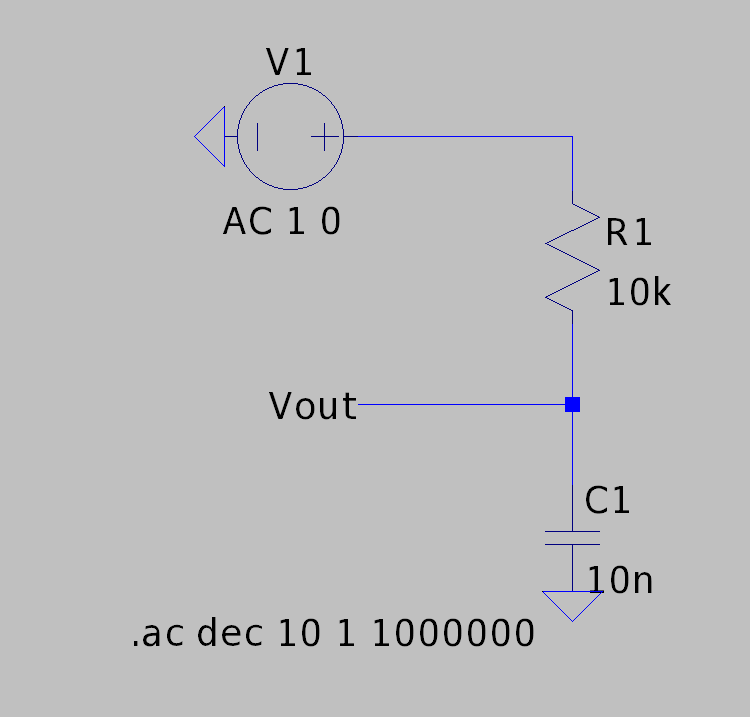
\includegraphics[width=0.5\textwidth]{first_order_schem}
		\caption{First-order Low Pass Filter circuit schematic.}
		\label{fig:first_order_schem}
	\end{figure}

	\begin{figure}[ht]
		\centering
		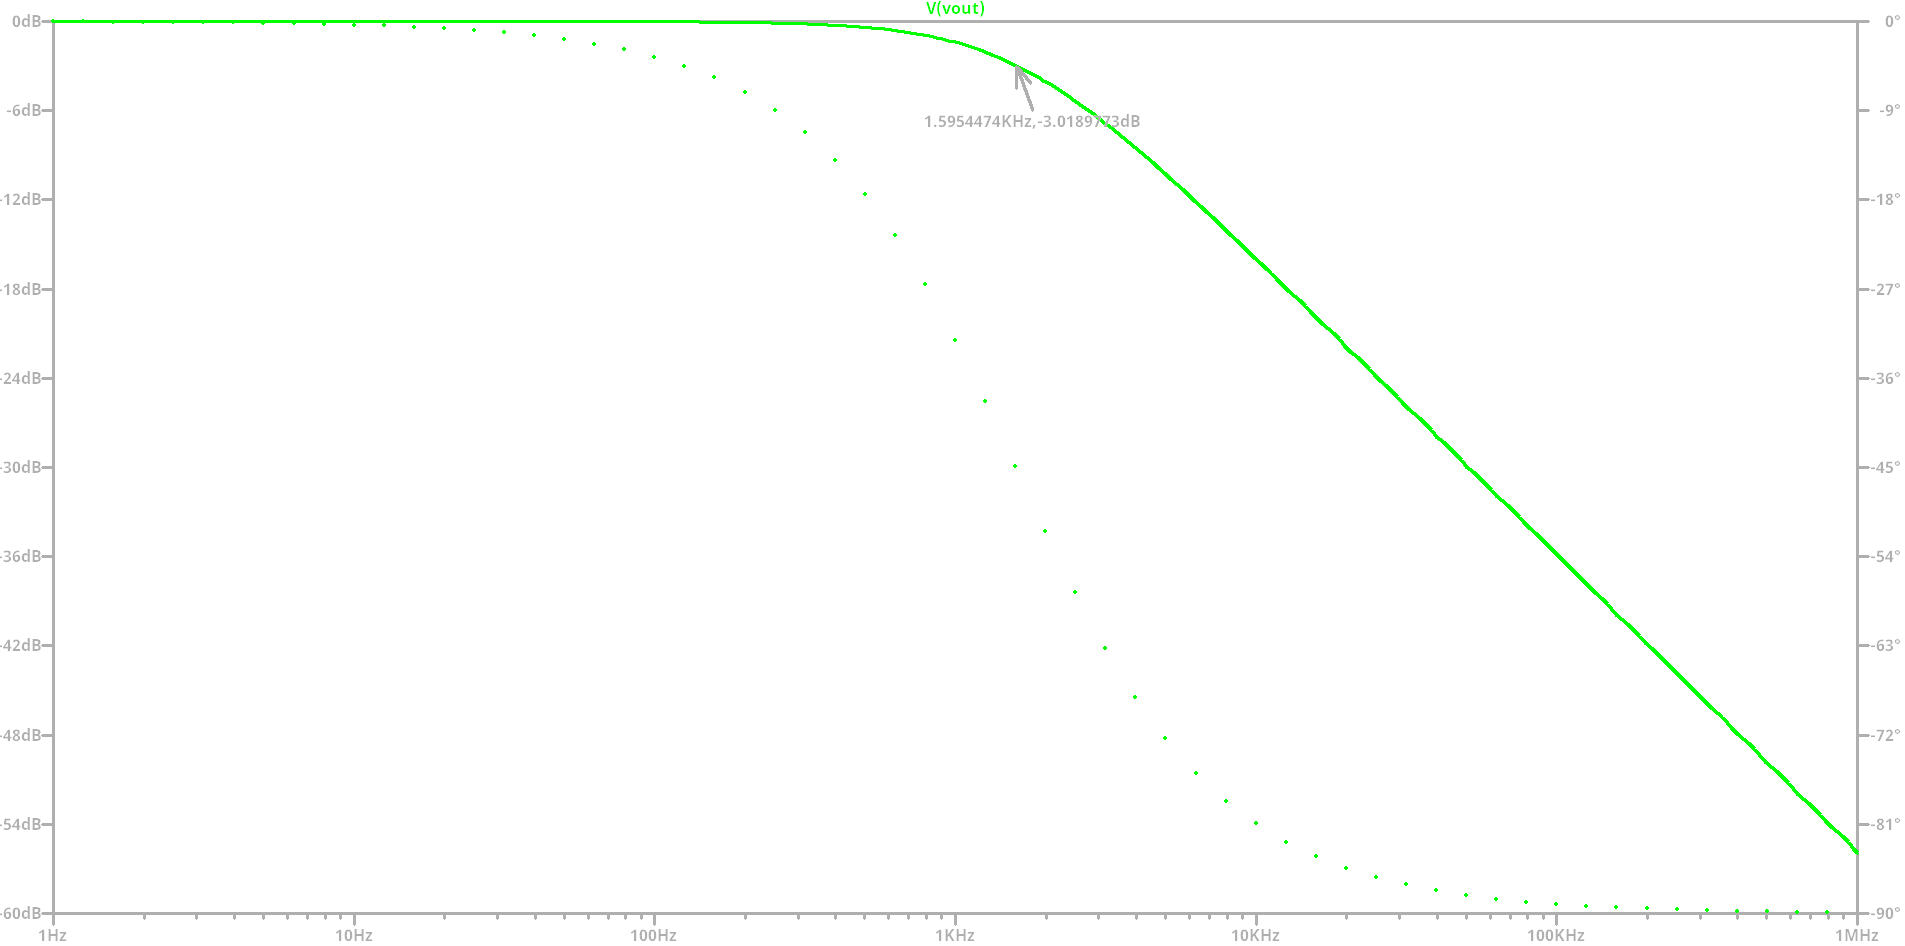
\includegraphics[width=0.8\textwidth]{first_order}
		\caption{First-order Low Pass Filter LT-Spice simulation from \SI{1}{\Hz} to \SI{1}{\mega\Hz}.}
		\label{fig:first_order}
	\end{figure}
	\pagebreak

	\subsection*{Second Order Low Pass Filter}
	\begin{figure}[ht]
		\centering
		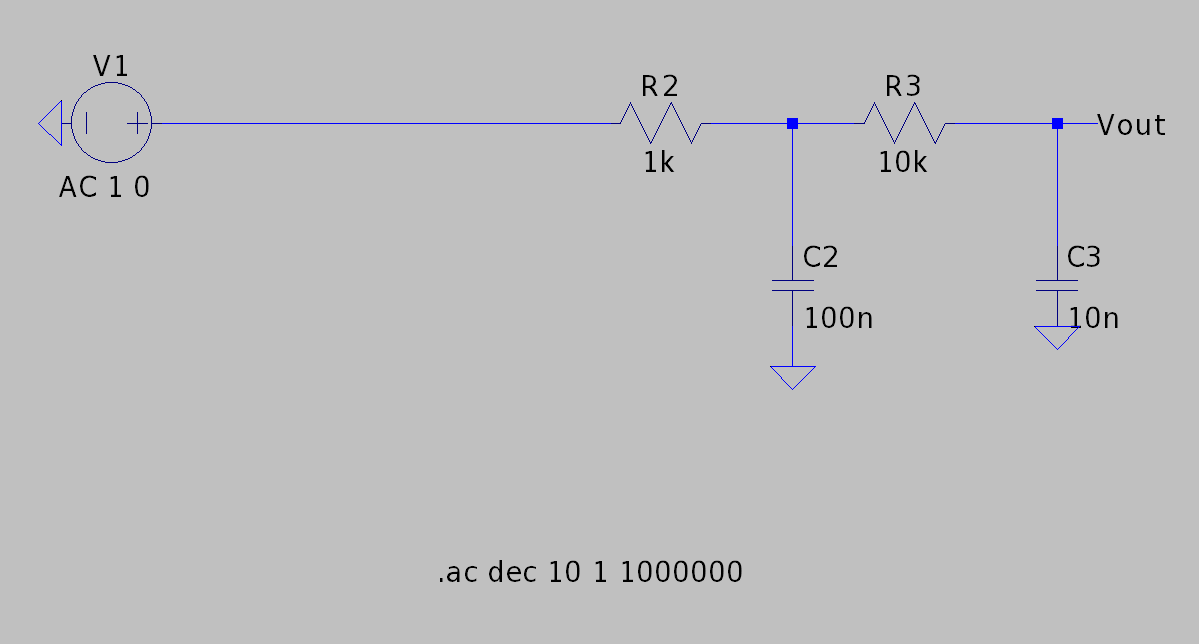
\includegraphics[width=0.6\textwidth]{second_order_schem}
		\caption{Second-order Low Pass Filter circuit schematic.}
		\label{fig:second_order_schem}
	\end{figure}

	\begin{figure}[ht]
		\centering
		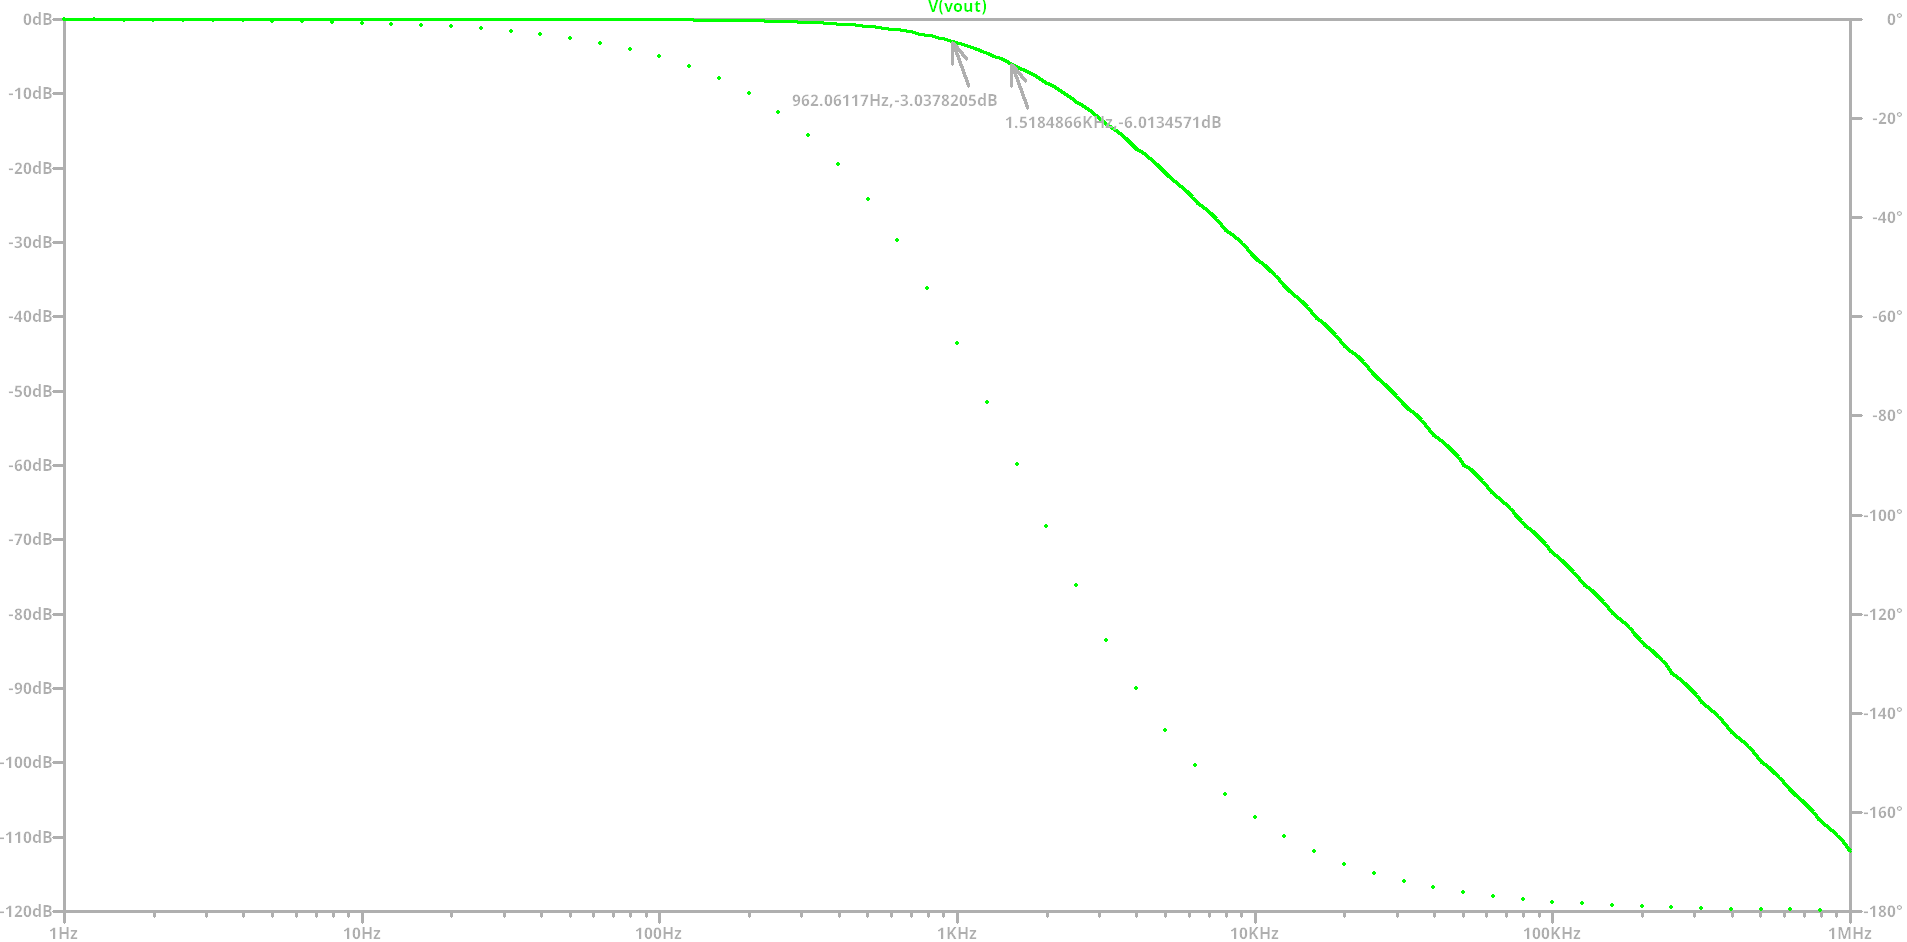
\includegraphics[width=0.8\textwidth]{second_order}
		\caption{Second-order Low Pass Filter LT-Spice simulation from \SI{1}{\Hz} to \SI{1}{\mega\Hz}.}
		\label{fig:second_order}
	\end{figure}
	\pagebreak

	\subsection*{Third Order Low Pass Filter}
	\begin{figure}[ht]
		\centering
		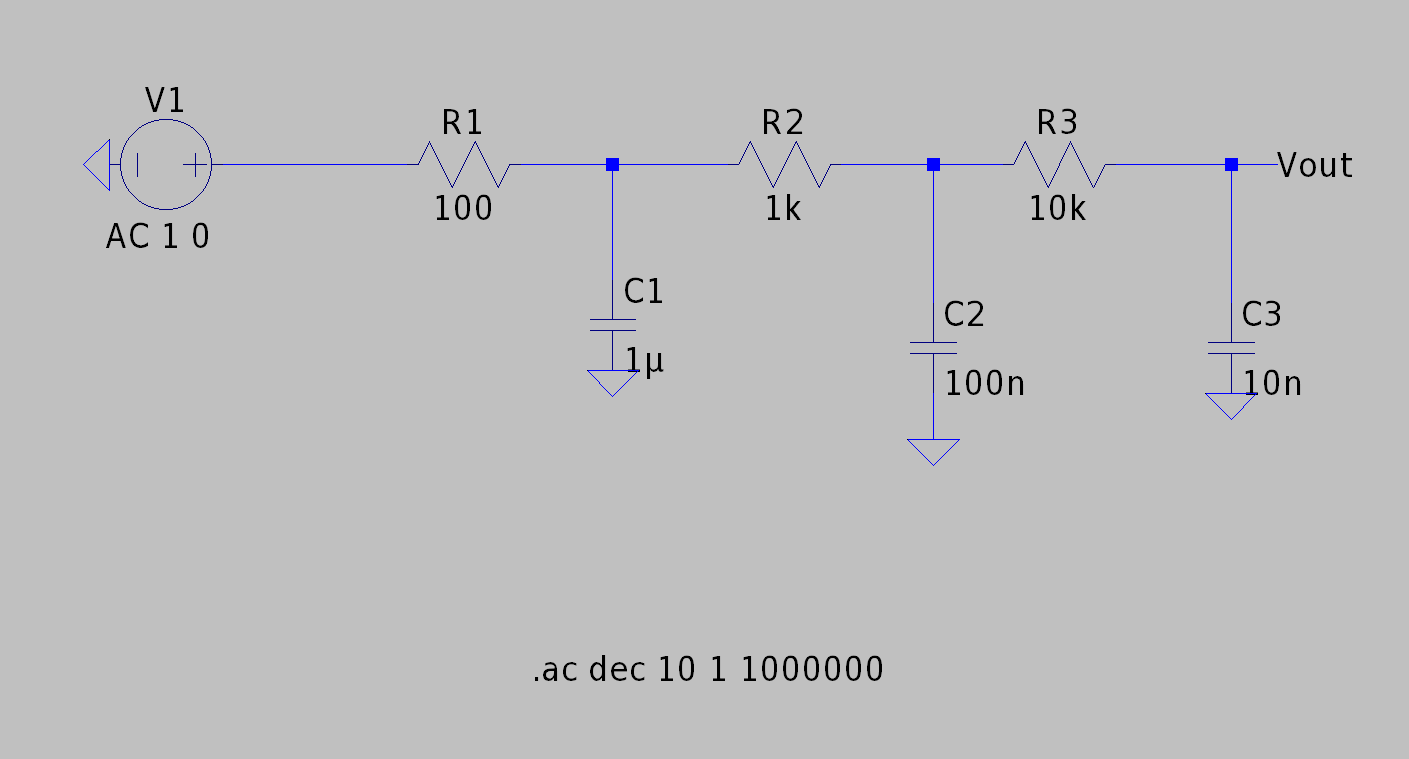
\includegraphics[width=0.6\textwidth]{third_order_schem}
		\caption{Third-order Low Pass Filter circuit schematic.}
		\label{fig:second_order_schem}
	\end{figure}

	\begin{figure}[ht]
		\centering
		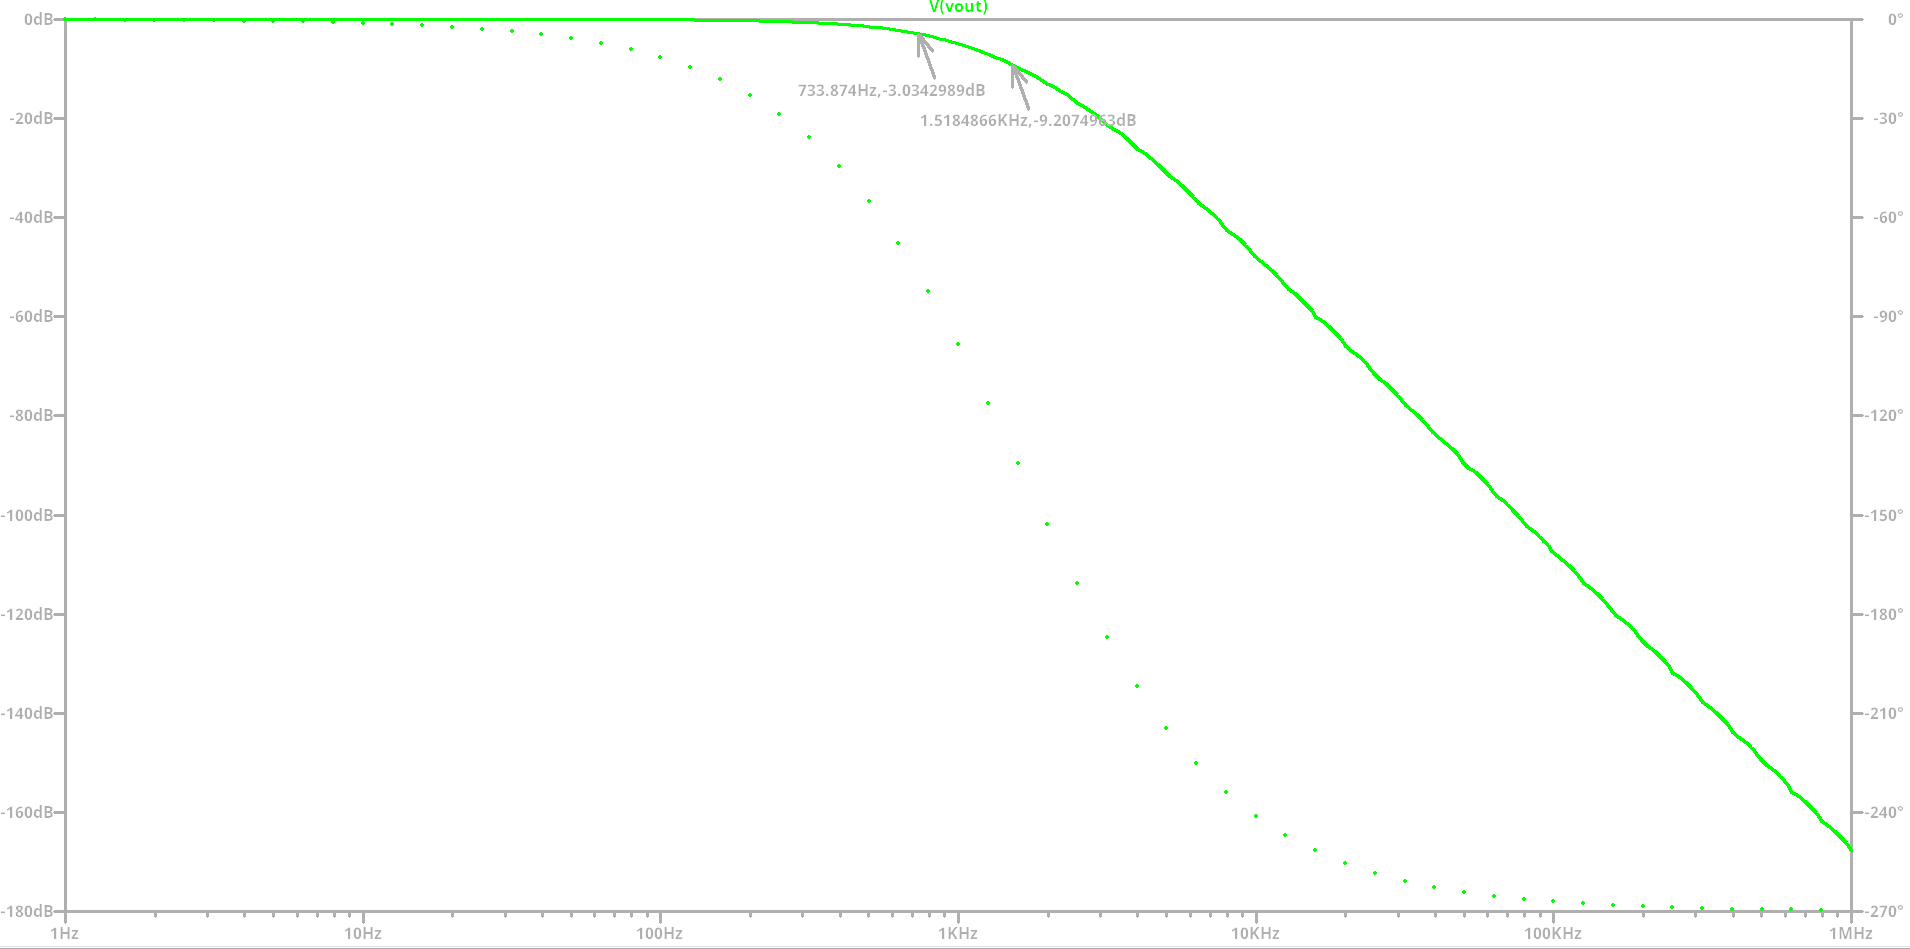
\includegraphics[width=0.8\textwidth]{third_order}
		\caption{Third Low Pass Filter LT-Spice simulation from \SI{1}{\Hz} to \SI{1}{\mega\Hz}.}
		\label{fig:third_order}
	\end{figure}

	\pagebreak

	\subsection*{First Order Low Pass Filter Parametric Sweep}
	\begin{figure}[ht]
		\centering
		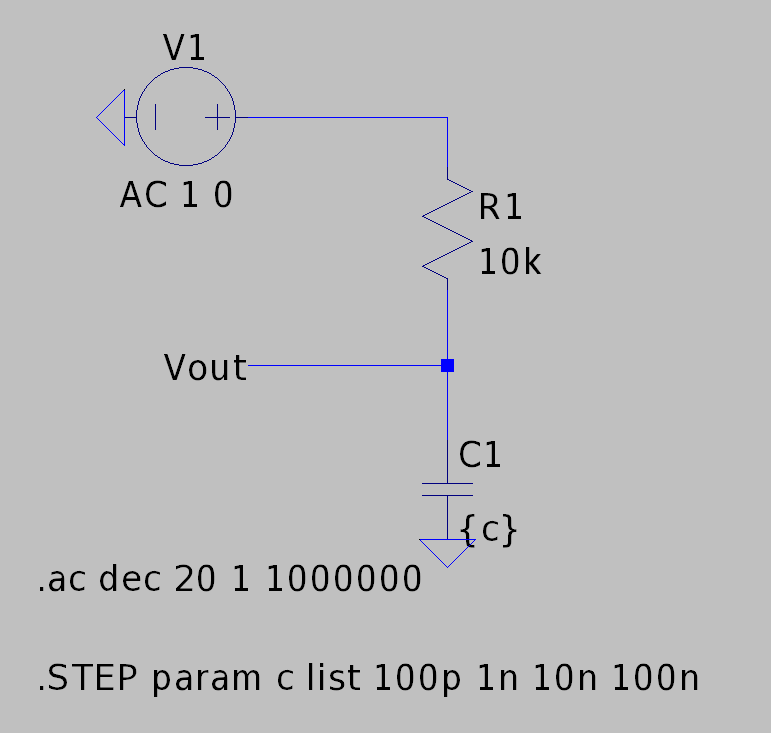
\includegraphics[width=0.5\textwidth]{low_pass_c_sweep_schem}
		\caption{Parametric sweep of low pass filter capacitor circuit schematic}
		\label{fig:parametric_sweep_schem}
	\end{figure}

	\begin{figure}[ht]
		\centering
		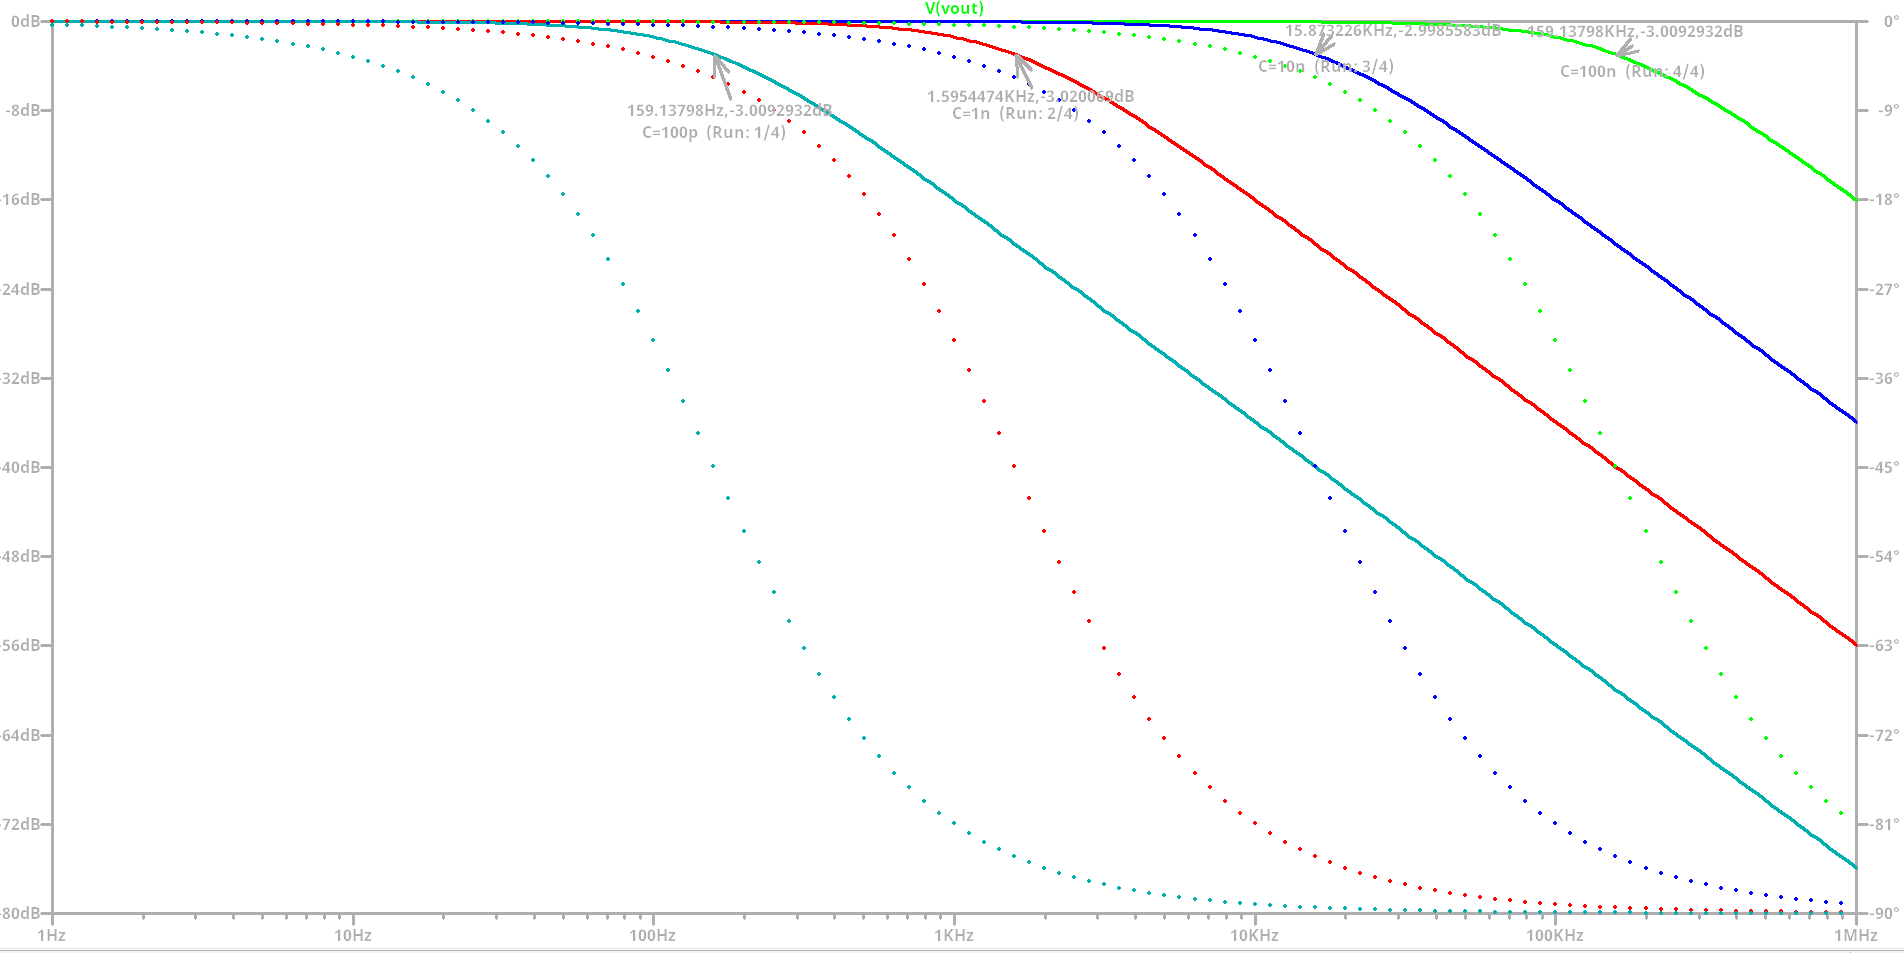
\includegraphics[width=0.8\textwidth]{low_pass_c_sweep}
		\caption{Parametric sweep of low pass filter capacitor LT-Spice simulation from \SI{1}{\Hz} to \SI{1}{\mega\Hz}.}
		\label{fig:parametric_sweep}
	\end{figure}

	\pagebreak

	\subsection*{Sallen-Key Low Pass Filter}
	\begin{figure}[ht]
		\centering
		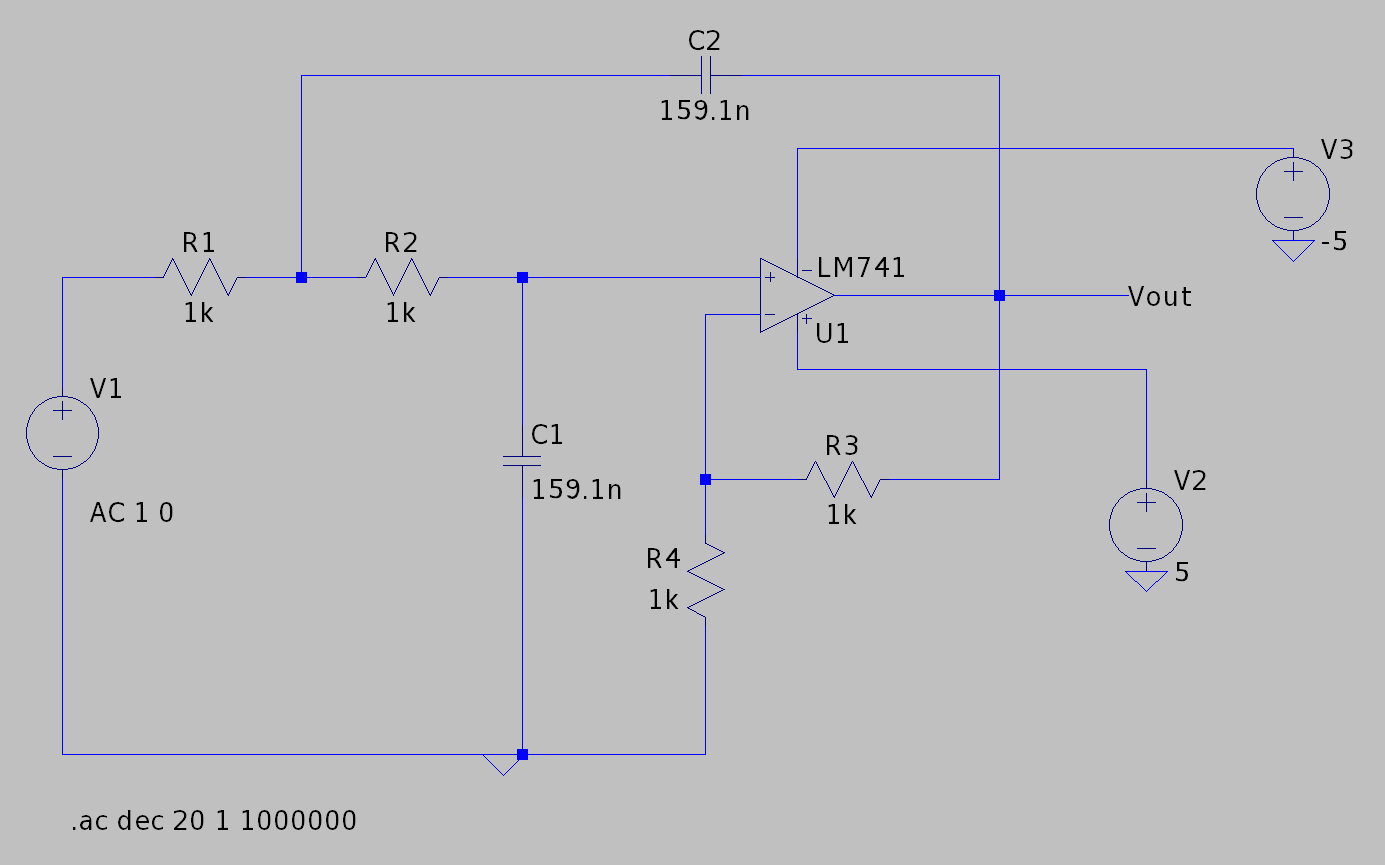
\includegraphics[width=0.7\textwidth]{sallen_key_schem}
		\caption{Sallen-Key Low Pass filter circuit schematic}
		\label{fig:sallen_key_schem}
	\end{figure}

	\begin{figure}[ht]
		\centering
		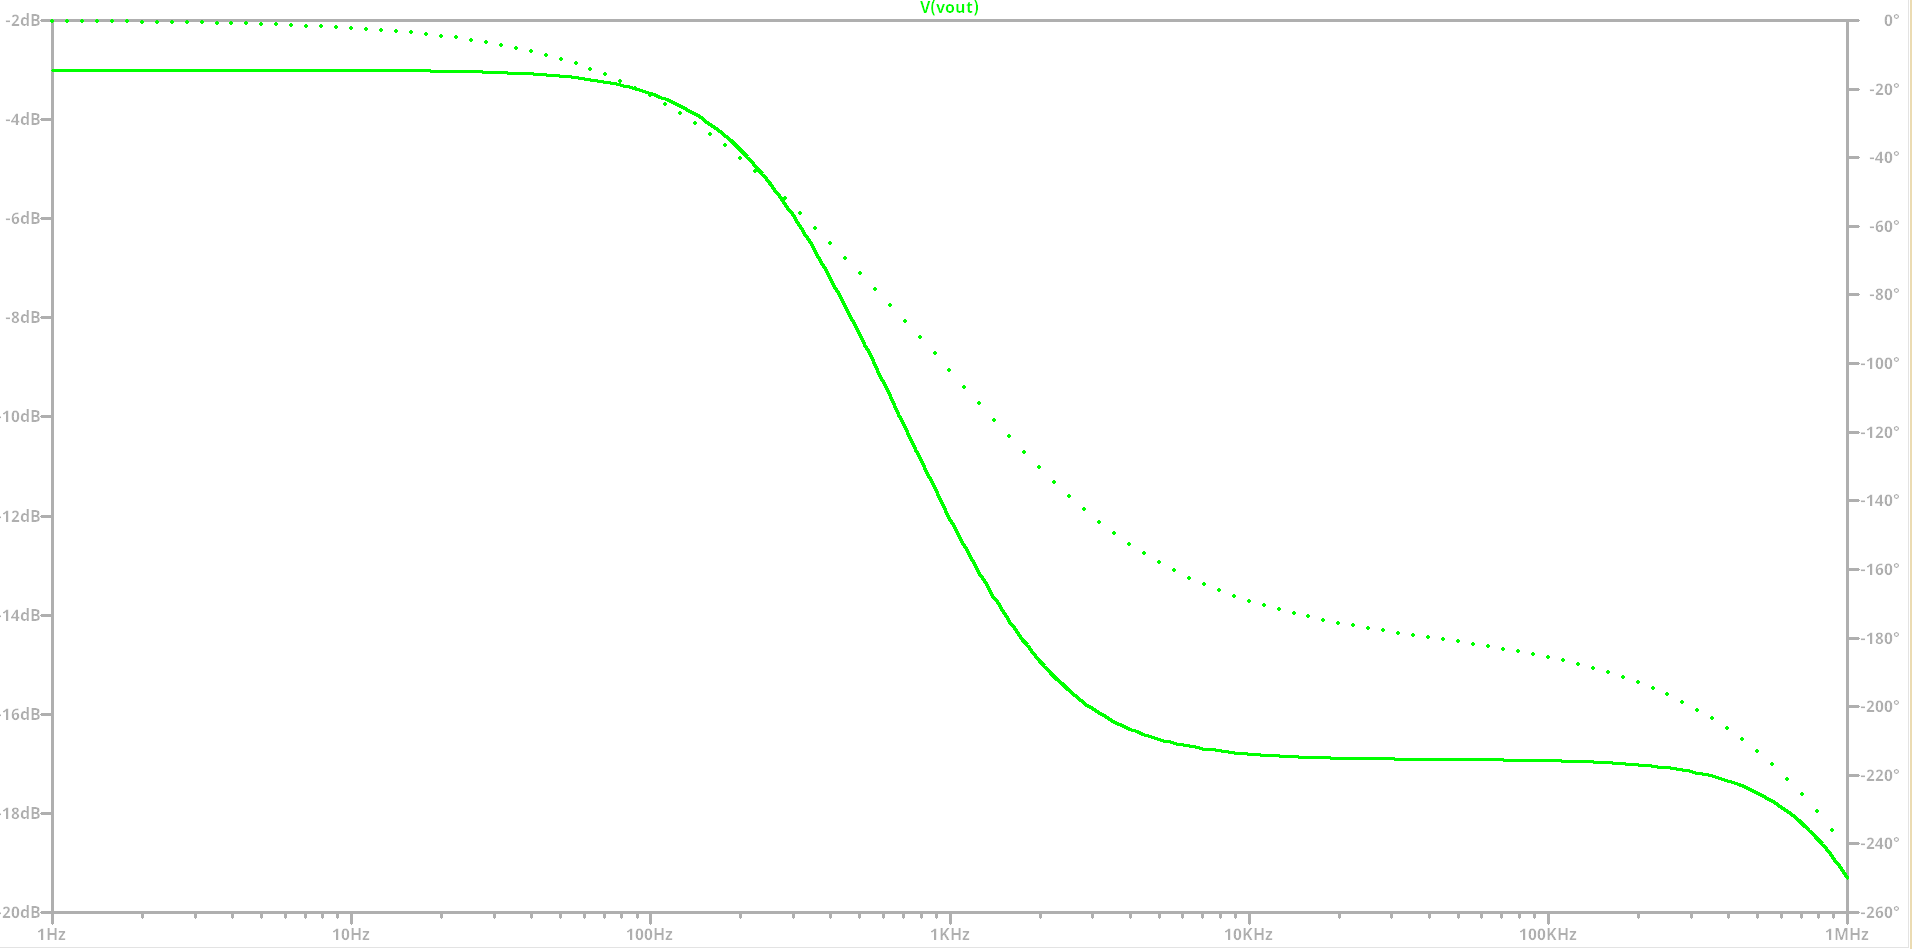
\includegraphics[width=0.8\textwidth]{sallen_key}
		\caption{Sallen-Key Low Pass filter LT-Spice simulation from \SI{1}{\Hz} to \SI{1}{\mega\Hz}.}
		\label{fig:sallen_key}
	\end{figure}

	\pagebreak

	\subsection*{Butterworth Low Pass Filter}
	\begin{figure}[ht]
		\centering
		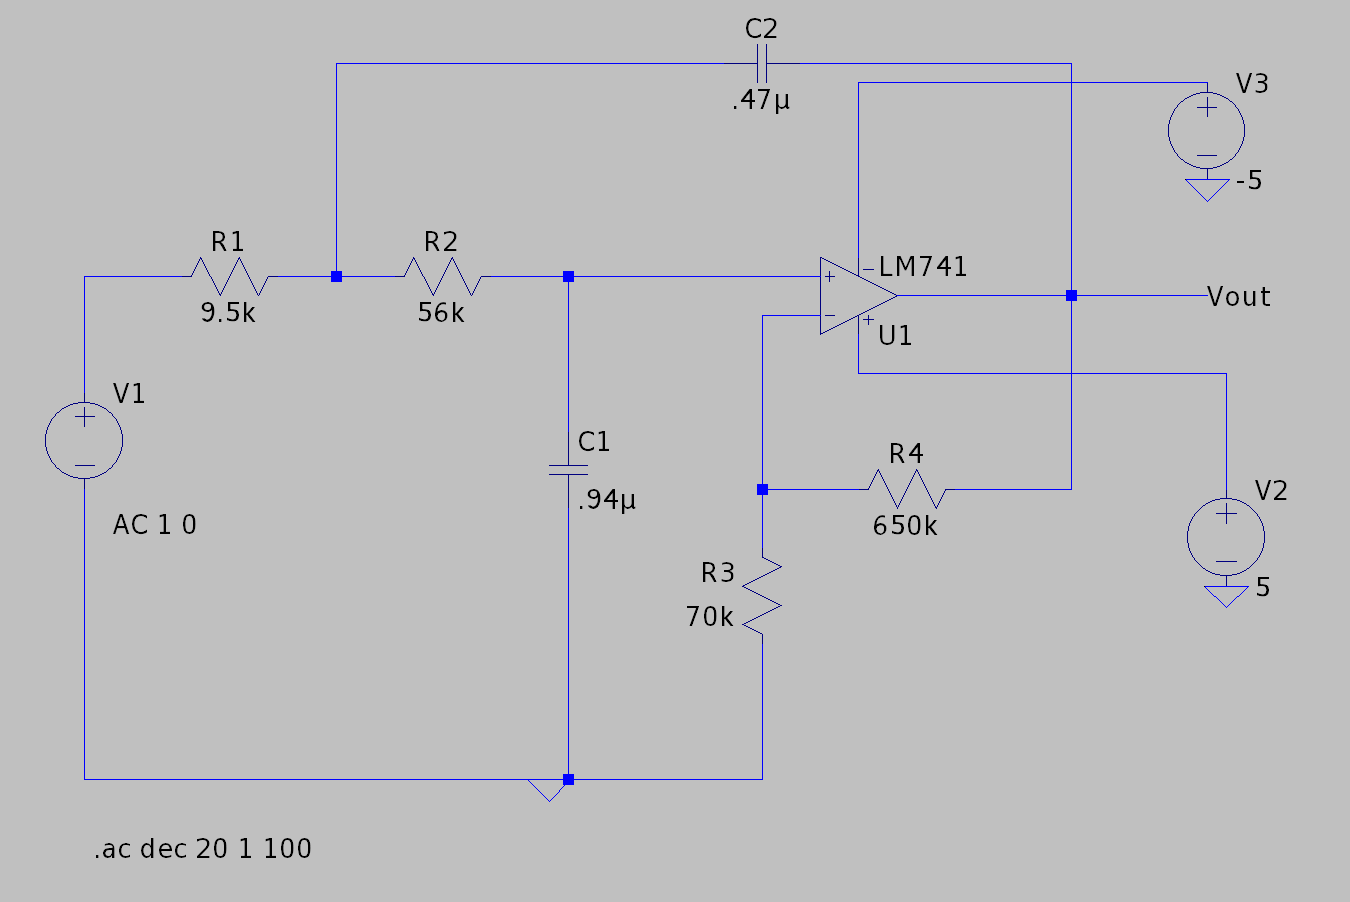
\includegraphics[width=0.7\textwidth]{butterworth_schem}
		\caption{Butterworth Low Pass filter circuit schematic}
		\label{fig:butterworth_schem}
	\end{figure}

	\begin{figure}[ht]
		\centering
		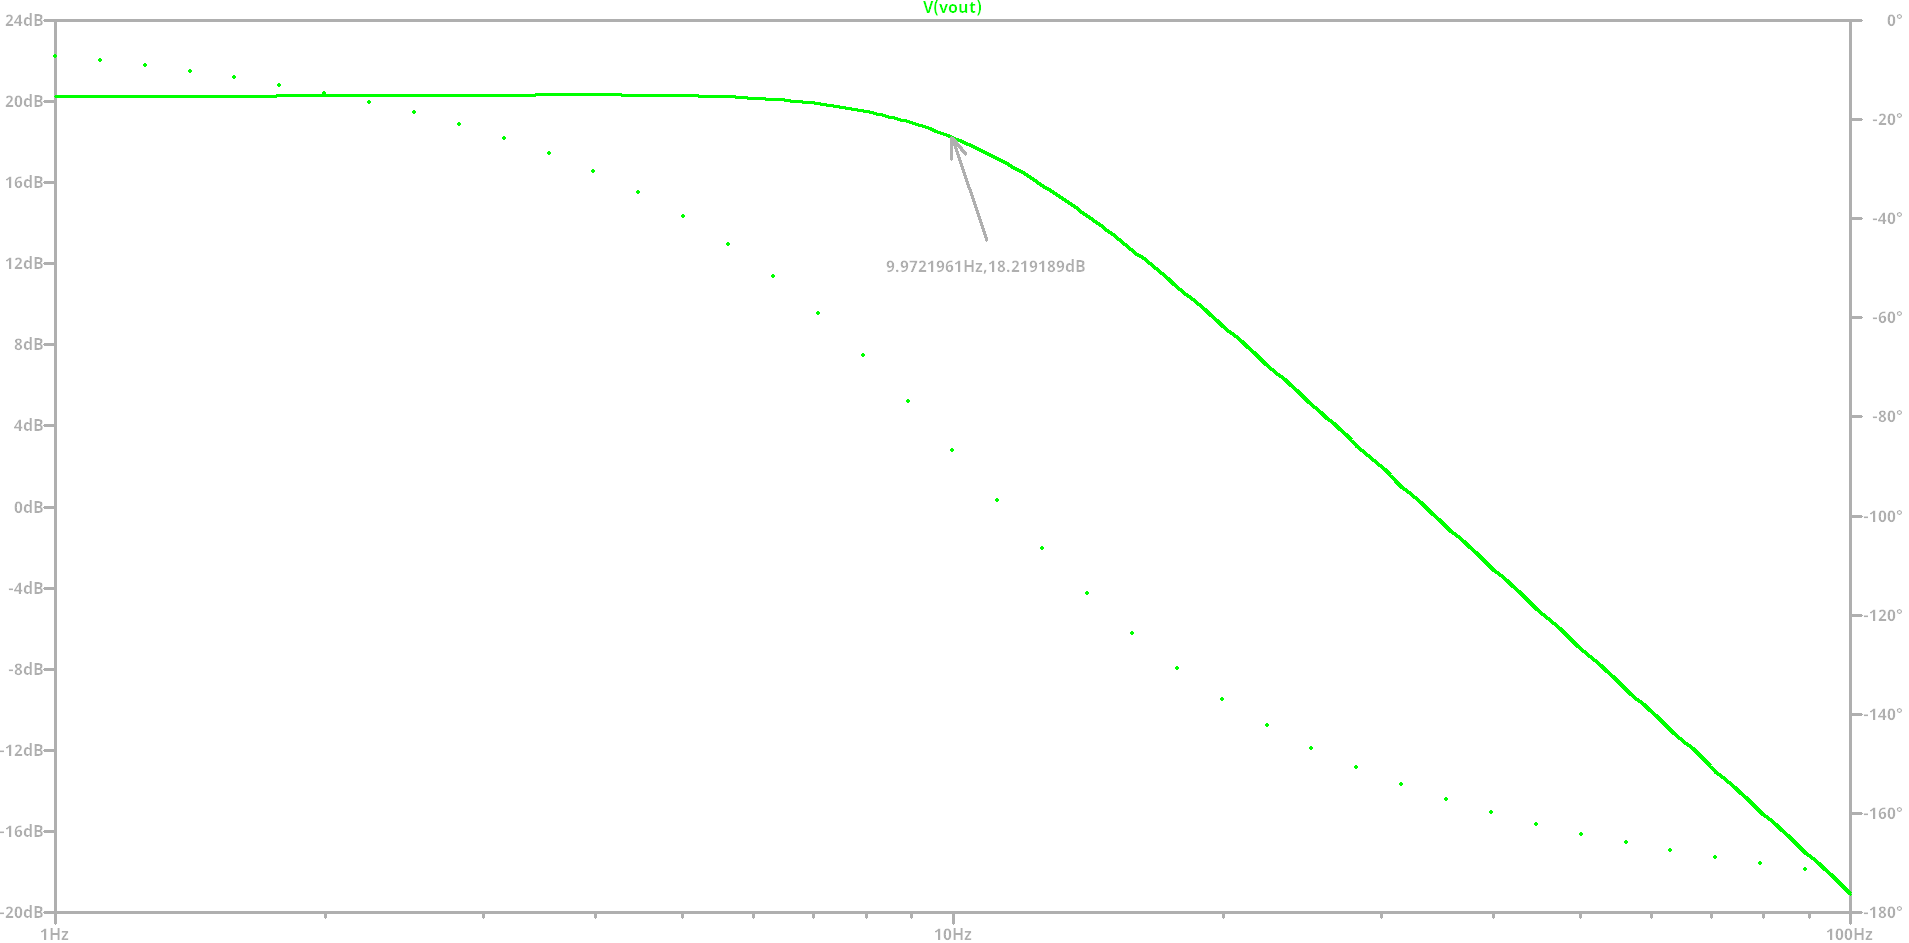
\includegraphics[width=0.8\textwidth]{butterworth}
		\caption{Butterworth LT-Spice simulation from \SI{1}{\Hz} to \SI{1}{\mega\Hz}.}
		\label{fig:butterworth}
	\end{figure}

	\pagebreak

	\subsection*{Bi-Quad Band Pass Filter}
	\begin{figure}[ht]
		\centering
		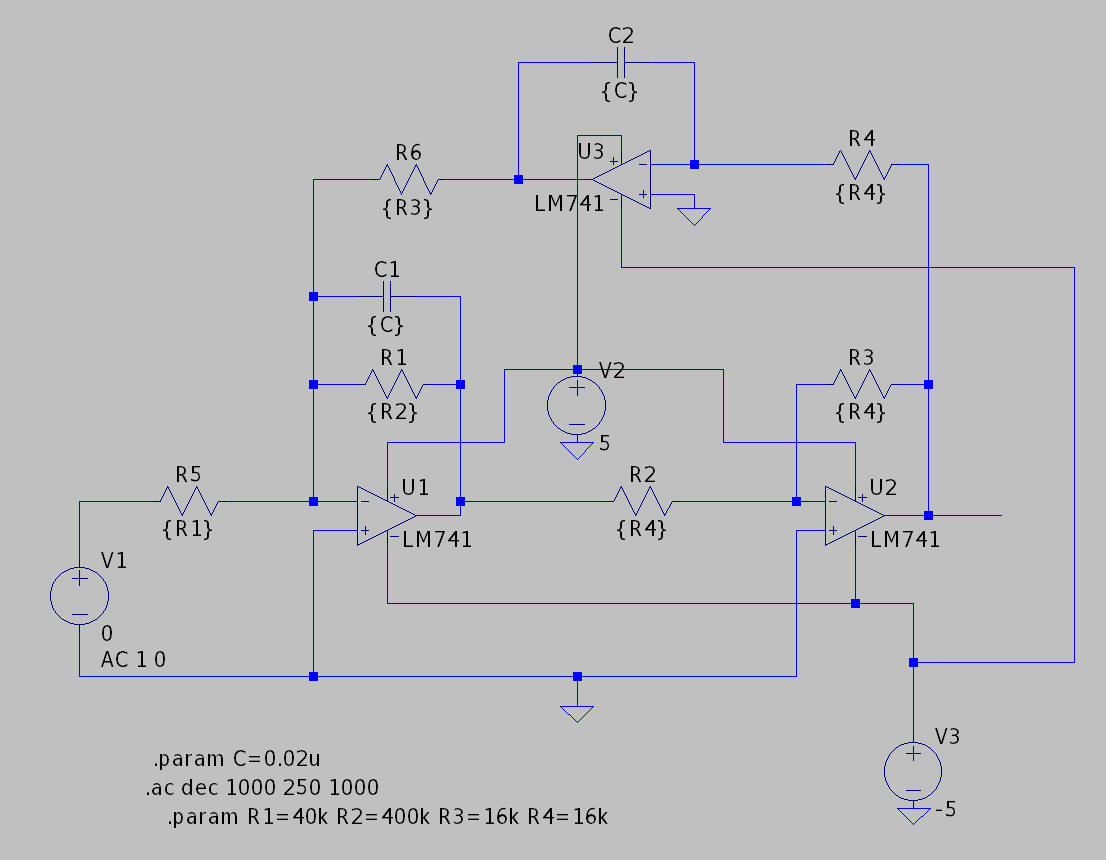
\includegraphics[width=0.6\textwidth]{band_pass_schem}
		\caption{Bi-Quad Band Pass filter circuit schematic (K=10)}
		\label{fig:band_pass_shem}
	\end{figure}

	\begin{figure}[ht]
		\centering
		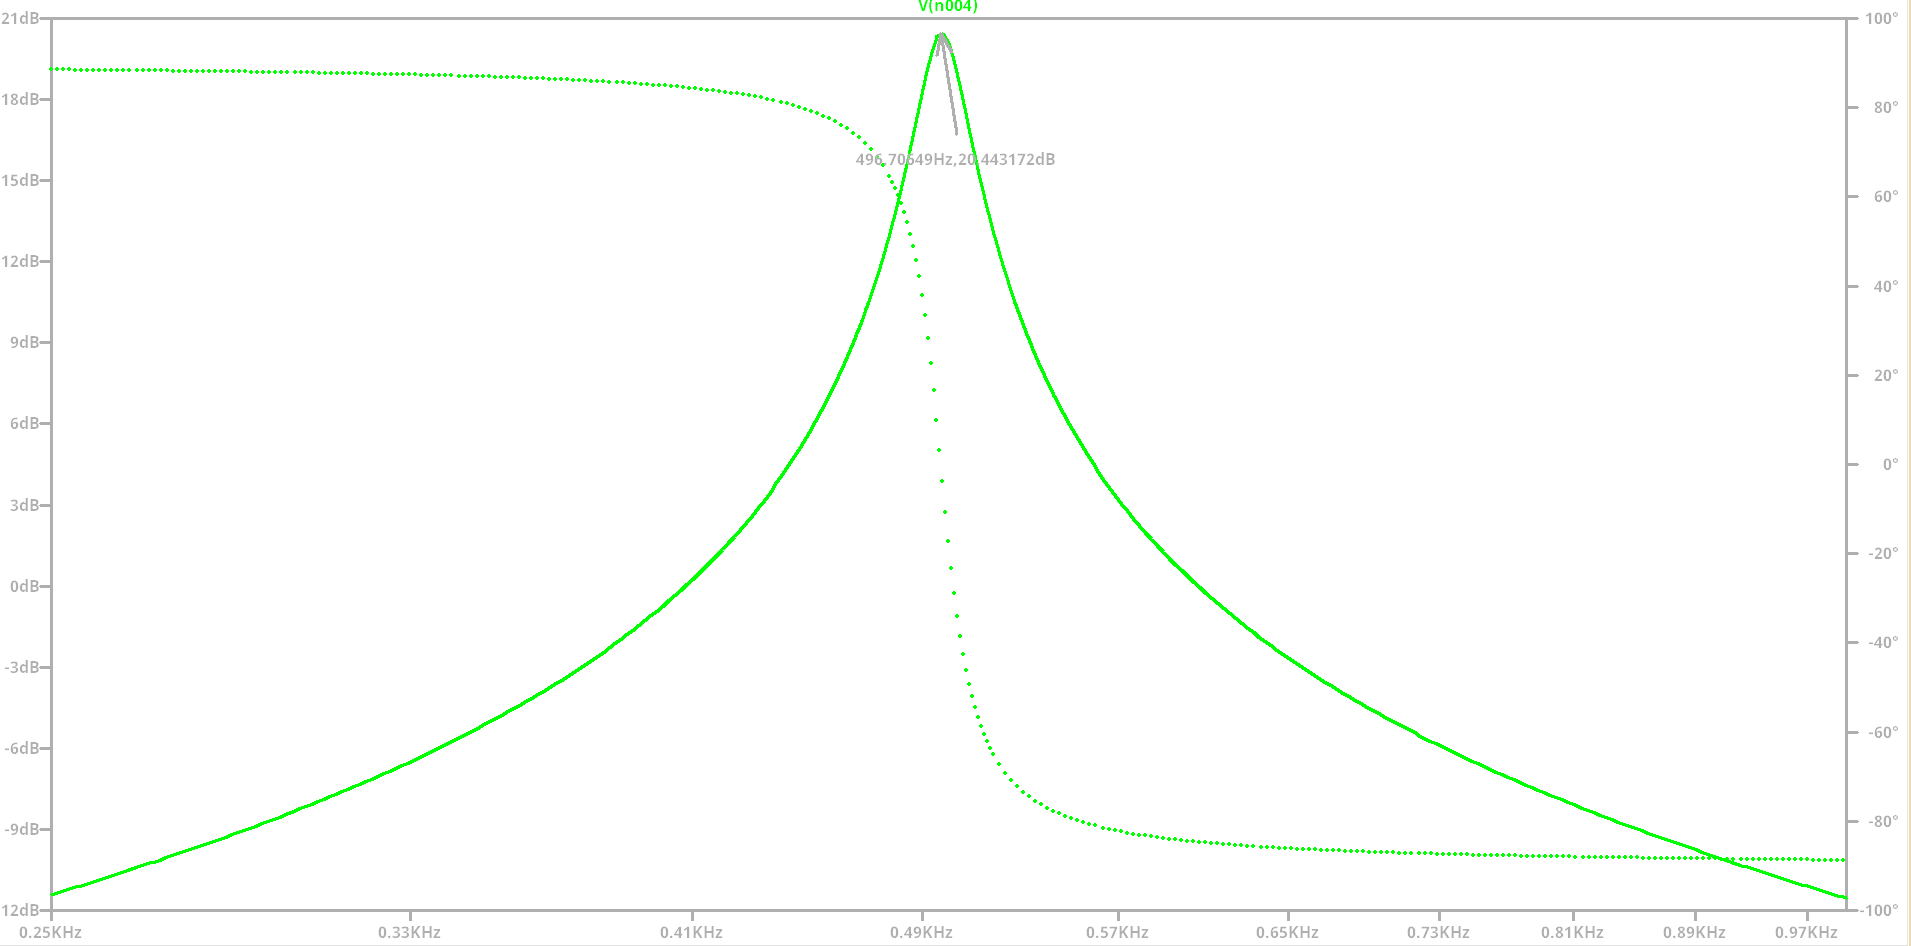
\includegraphics[width=0.8\textwidth]{band_pass}
		\caption{Bi-Quad Band Pass Filter LT-Spice simulation from \SI{1}{\Hz} to \SI{1}{\mega\Hz}.}
		\label{fig:band_pass}
	\end{figure}

	\pagebreak

	\section*{In-lab questions}

	\begin{enumerate}
	\item{ What is the slope of each of the (straight line portion) of each magnitude plot curve?}

	\SI{-40}{\dB \per decade}
	

	\item{What would happen as more stages are added?}

	If more low pass filter stages were added, the linear portion would approach a vertical
	line (brick wall). Each extra stage adds \SI{-40}{\dB \per decade} to this slope.

	\item{Can you think of an ideal component/circuit to put between each stage?}

	A voltage follower can be used to completely isolate the input reactance of the
	filter stages from each other.

	\end{enumerate}

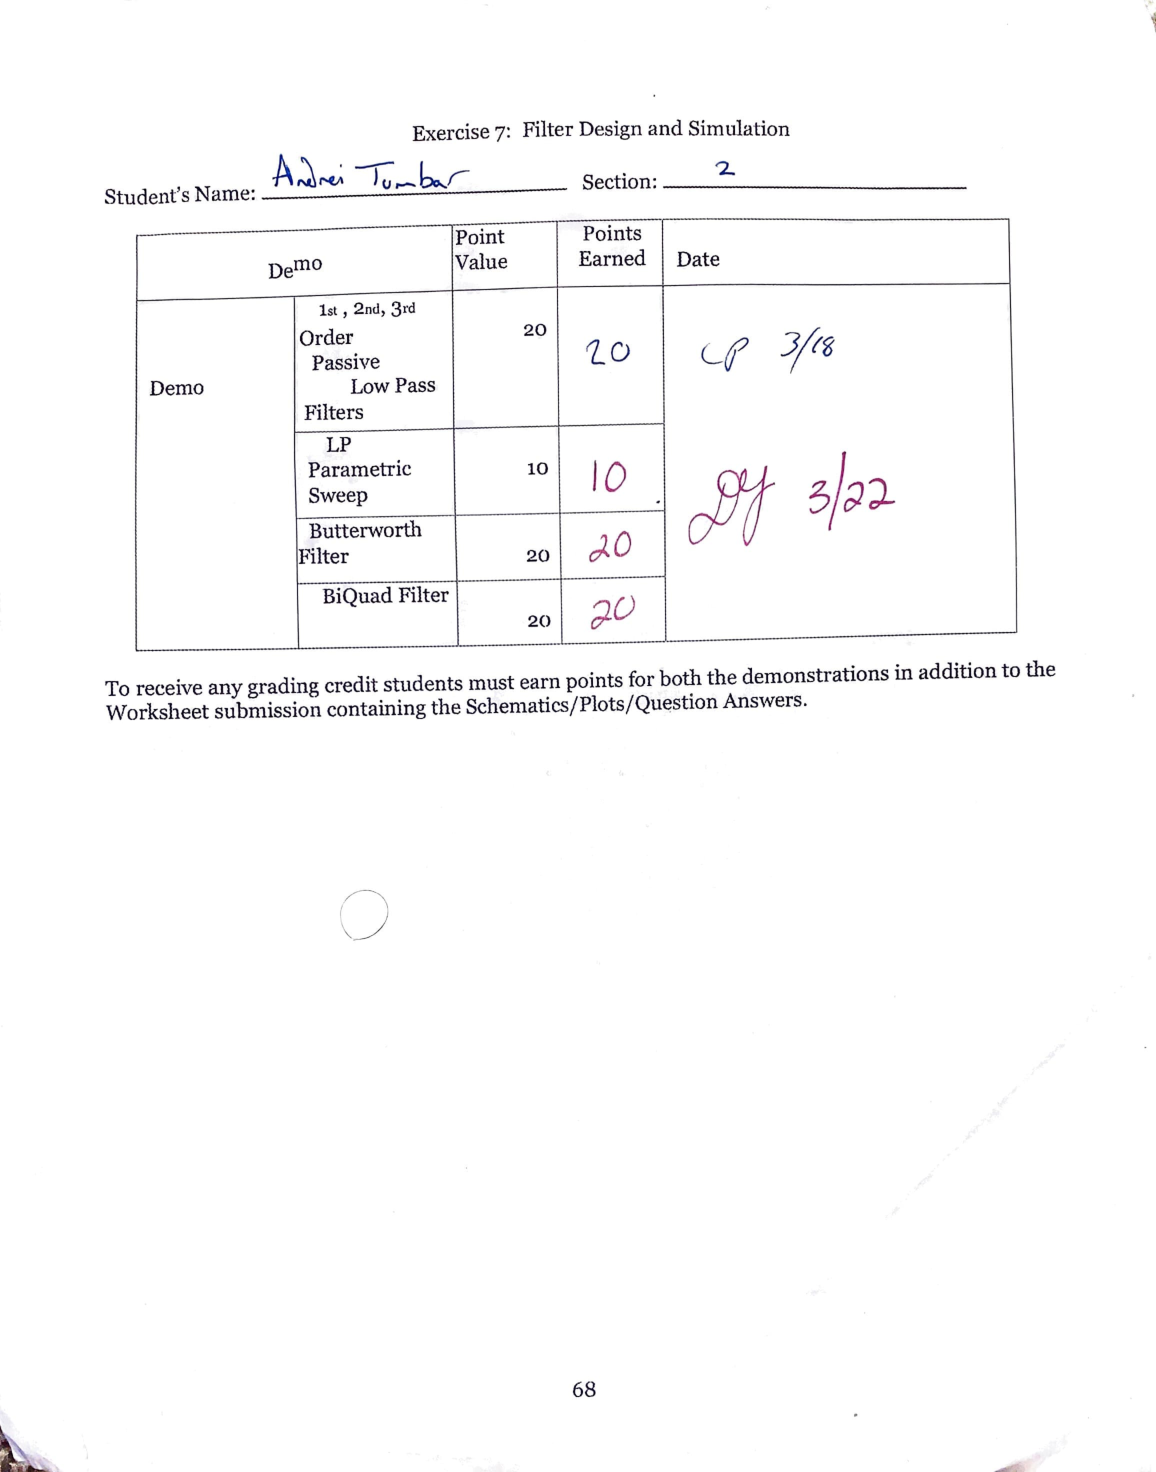
\includepdf[pages=-,pagecommand={},width=\textwidth]{signoff7.pdf}

\end{document}
